%%%%%%%%%%%%%%%%%%%%%%%%%%%%%%%%%%%%%%%%%%%%%%%%%
% Adam Wright
% Background
% back.tex
%%%%%%%%%%%%%%%%%%%%%%%%%%%%%%%%%%%%%%%%%%%%%%%%%%
\chapter{Background}
Laser guide stars (LGS)\footnote{LGS will refer to both the plural and singular of the word, e.g. ``LGS are frequently used in modern astronomy'' and ``LGS systems consist of many components.'' Context should provide the correct form throughout reading this thesis.}  are invaluable instruments in modern astronomy, allowing observations of extremely high resolution to be made even in unfavorable atmospheric conditions. An important quality of an LGS is its brightness, which affects the overall performance of the adaptive optics system and limits the resolution that the telescope can achieve. However, taking advantage of the atoms' precession in a magnetic field, the brightness of LGS can be increased through magnetic resonant pulsing (MRP). In this chapter, we describe the quantum theory behind LGS and magnetic resonant pulsing.

\section{Quantum Theory of Laser Guide Stars}


%In a simple model, the electrons in the atom are ``orbiting'' the nucleus. This model, proposed by Niels Bohr in the early twentieth century, is known as the \textit{Bohr Model}. The electrons orbit in discrete radii of quantized energy, or shells, each of which is denoted by the principal quantum number $n = 1,2,3,\dots$. Each electron shell refers to a certain energy of the atom, and electrons are free to transition between shells as long as energy is conserved during this transition.\footnote{Other quantities, such as angular momentum, must also be conserved. These will be addressed shortly.} As a pedagogical example, we can calculate the energy needed for an electron transitioning between shells in hydrogen using the famous Rydberg formula
%
%\begin{equation}
%  \Delta E = hc R_H\left( \frac{1}{n_f^2} - \frac{1}{n_i^2}\right),
%  \label{rydberg}
%\end{equation}
%%
%where $h$ is Planck's constant, $c$ is the speed of light in a vacuum, $R_H = \SI{1.1e7}{\per\meter}$ is the Rydberg constant for hydrogen, $n_f$ is the principal quantum number of the final state, and $n_i$ is the principal quantum number of the initial state. Empirically, we see that atoms emit photons (i.e. particles of light) when they decay from states of higher energy to those with lower energy. Furthermore, the energy of these emitted photons is exactly equal to the energy difference between these two states. Knowing that the energy of a photon is
%
%\begin{equation}
%  E = h f = \frac{hc}{\lambda},
%  \label{energyfrequency}
%\end{equation}
%%
%where $f$ is the frequency of the photon, and $\lambda$ is the wavelength of the photon, we can calculate the wavelength of light a transition would emit using this and Eq. \ref{rydberg},
%
%
%\begin{equation}
%		\frac{1}{\lambda} = R\left( \frac{1}{n_f^2} - \frac{1}{n_i^2}\right).
%  \label{rydbergw}
%\end{equation}
%%
%Thus, if we wanted to know the wavelength of a photon that is emitted when an electron in the $n_i=1$ shell is completely ejected from the atom (ionization), we could compute this by letting $n_f = \infty$ and find that $\lambda_{L_{\infty}} = $ \SI{91}{\nano \meter} (this is one transition in the well known Lyman series \cite{Townsend}). This process is also reversible, meaning an atom can be excited by absorbing a photon of wavelength equal to this calculated wavelength. The wavelength of light needed for this excitation is known as the resonant wavelength. This is the foundation of LGS --- laser light resonant with sodium is shone onto sodium atoms in the atmosphere, the atoms absorb light, and then emit this light in random directions, creating a ``globe'' of light (see Appendix A for a discussion of laser guide stars). The Bohr model, however, is not accurate, especially for atoms of more than one electron. 

In order to fully describe the physics of the atoms, \textit{quantum mechanics}, the branch of physics that concerns itself with describing the behavior of particles and energies of the smallest scales, is needed. The fundamental equation in quantum mechanics is the Schr\"{o}dinger equation, which details how a quantum system will evolve and is given by

\begin{equation}
	i \hbar \frac{\partial}{\partial t} \left| \psi(\vec r,t) \right> = \hat H \left| \psi (\vec r,t)\right>,
	\label{eq:schrodingers}
\end{equation}
%
where $i = \sqrt{-1}$, $\hbar = \frac{h}{ 2 \pi}$ is the reduced Planck's constant, $\psi (\vec r,t)$ is the spatially and temporally dependent wavefunction of the particle, and $\hat H$ is the Hamiltonian operator, describing the energy of the system. For a particle in a time-independent system with a central potential dependent upon $r$, the wave function $\psi (\vec r)$ can be separated into three functions each of which describes a particular coordinate 

\begin{equation}
	\psi(r, \theta, \phi) = R(r) \Theta(\theta) \Phi(\phi), 
	\label{eq:seppsi}
\end{equation}
%
where $R(r)$ is the radial function, $\Theta(\theta)$ is the polar function, and $\Phi(\phi)$ is the azimuthal function.\footnote{It is common for $\Theta$ and $\Phi$ to be combined into one function, which can be written in terms of the spherical harmonics $Y^m _L$ described by the quantum numbers $L$ and $m_L$ \cite{Townsend}.} Substituting Eq. \ref{eq:seppsi} into Eq. \ref{eq:schrodingers}, the spatial functions $R(r)$, $\Theta(\theta)$, and $\Phi(\phi)$ can each be solved separately. In order to solve them, however, three quantum numbers are introduced: the principal quantum number $n$ (introduced earlier), coming from the radial function of the Schr\"{o}dinger equation; the orbital angular momentum quantum number $L$, coming from the polar function; and the magnetic quantum number $m_L$, coming from the azimuthal function.


It was later realized that a fourth quantum number, known as spin\footnote{Spin was empirically discovered through the famous Stern-Gerlach experiment in 1922 where silver atoms were deflected by an inhomogeneous magnetic field depending on their spin \cite{Townsend}.} and denoted $S$, was needed in order to fully describe the behavior of many particles. Spin describes a particle's intrinsic (spin) angular momentum and takes on full or half integer values of the reduced Planck's constant $\hbar$. For example, electrons are spin-$\frac{1}{2}$ particles and thus have a $z$-component of spin $S_z = \pm \frac{\hbar}{2}$, while photons are spin-$1$ particles with $S_z = \pm \hbar$. 

When all of these quantum numbers are considered collectively, we find interesting phenomena occurring in the energies of atoms. Upon first inspection, we see that many energy levels actually consist of multiple, closely-spaced sublevels. These sublevels are caused in part by the relativistic energy of the particles and in part by the interaction between the electron's spin and its orbital angular momentum. Spin, being a value of the intrinsic angular momentum, can couple with the \textit{orbital} angular momentum, causing an interaction that shifts and splits each energy level. The relativistic energy simply shifts the value of the energy level by more accurately describing the particle's kinetic energy. Collectively, these corrections are known as the \textit{fine structure} \cite{Kibblewhite2009}. The spin-orbit coupling follows the formula 

\begin{equation}
  \vec J = \vec L + \vec S,
  \label{fineequation}
\end{equation}
%
where $\vec J$ is the total angular momentum vector, $\vec L$ is the orbital angular momentum vector with magnitude $|\vec L| = \hbar \sqrt{L (L + 1)}$, and $\vec S$ is the spin angular momentum vector with magnitude $|\vec S| = \hbar \sqrt{S(S+1)}$. The values that the splitting can thus take are $|J| = |L - S|, \dots, |L +S|$ in integer steps. Thus, for a state of $L=0$ with a particle of spin-$\frac{1}{2}$, $J = |0-\frac{1}{2}|, \dots, |0+\frac{1}{2}| = \frac{1}{2}$, indicating there being only an energy shift and not split. However, for the $L=1$ state, $J = |1-\frac{1}{2}|,\dots, |1+\frac{1}{2}| = |-\frac{1}{2}|, \dots, |\frac{3}{2}| =  \frac{1}{2}, \frac{3}{2}$, indicating a two--fold split.


We can look even more carefully at the energy levels of atoms. We saw how the spin $\vec S$ interacted with the orbital angular momentum $\vec L$ to cause an energy split, but the total angular momentum $\vec J$ can also interact with the spin of the nucleus, causing yet another, even smaller\footnote{For hydrogen, these shifts are on the order of millionths of an electronvolt \cite{feynman}. Compared with the ionization energy of $13.6 \text{ eV}$, this is quite small.} splitting of the energy levels. This is the \textit{hyperfine structure} and follows the formula

\begin{equation}
\vec F = \vec J + \vec I,
  \label{hyperfine}
\end{equation}
%
where $\vec F$ is the new total angular momentum vector and $\vec I$ is the nuclear spin.\footnote{This splitting holds true for atoms with relatively low atomic number, including the atoms we are studying (rubidium and sodium). Heavier atoms couple differently.} The splitting obeys $F = |J-I|, \dots, |J+I|$, causing degeneracy for all states with $J \neq 0$ and $I \neq 0$.

Finally, if we consider the atom to be in a magnetic field, we observe another splitting known as the \textit{Zeeman effect}. The Zeeman effect results from a magnetic field interacting with $\vec F$, causing a precession of this vector about the axis of the magnetic field. The energy shift follows the equation

\begin{equation}
  \Delta E = \mu_B m_F g_F B,
  \label{zeeman}
\end{equation}
%
where $\mu_B$ is the Bohr magneton, $m_F$ is the $z$-component of the total angular momentum, $g_F$ is the Land\'{e} $g$-factor,\footnote{The Land\'{e} $g$-factor is a particular g-factor (a dimensionless number describing the magnetic moment) that accounts for both the spin and orbital angular momentum of the particle. It is described mathematically as 
  \begin{equation}
	g_F = g_J \frac{F(F+1) -I(I+1) + J(J+1)}{2F(F+1)} + g_I \frac{F(F+1) + I(I+1) -J(J+1)}{2F(F+1)},
	\label{lande}
  \end{equation}
%
where $g_{J,I}$ are the Lande g-factors for the those particular quantum values, and $F,J,$ and $I$ are the quantum values discussed earlier.} and $B$ is the magnetic field. The splitting is quantized by the values of the $z$-component of the orbital angular momentum, $m_F = -F, \dots, F$. Since sodium, the basis of LGS systems, exists within the geomagnetic field and has a magnetic moment, its energy levels are split due to the Zeeman effect.

Bringing everything together, we can show these energy shifts and splits schematically, as in Fig. \ref{fig:energysplitting} for the case of $I = 3/2$. From left to right, the order of magnitude of the splitting gets smaller. The scale of the fine structure splitting is $Z \alpha^2$, where $Z$ is the atomic number and $\alpha = 1/137$ is the fine structure constant \cite{feynman}. The scale of the hyperfine structure is typically an order of magnitude smaller than the fine structure, and the Zeeman split is typically an order of magnitude smaller than the hyperfine split. As we move up vertically, we get varying levels of splitting depending on the quantum number involved. 

\begin{figure}[ht]
	\centering
	\includestandalone{Images/tikz/quantumstructure}
	\caption{Shown is the  splitting of energy levels due to the fine, hyperfine, and Zeeman effect with principal quantum number $n$, angular momentum quantum number $L$, total angular momentum quantum number $J$, total atomic angular momentum quantum number $F$, and magnetic quantum number $m_F$ for the case of $I = 3/2$ (not all Zeeman splits are shown).}
  \label{fig:energysplitting}
\end{figure}


%%%%%%%%%%%%%%%%%%%%%%%%%%%%%%%%%%%%%%%%%%%%%%%%%%
% Sodium transitions
%%%%%%%%%%%%%%%%%%%%%%%%%%%%%%%%%%%%%%%%%%%%%%%%%%
%\begin{figure}[ht!]
%  \centering
%  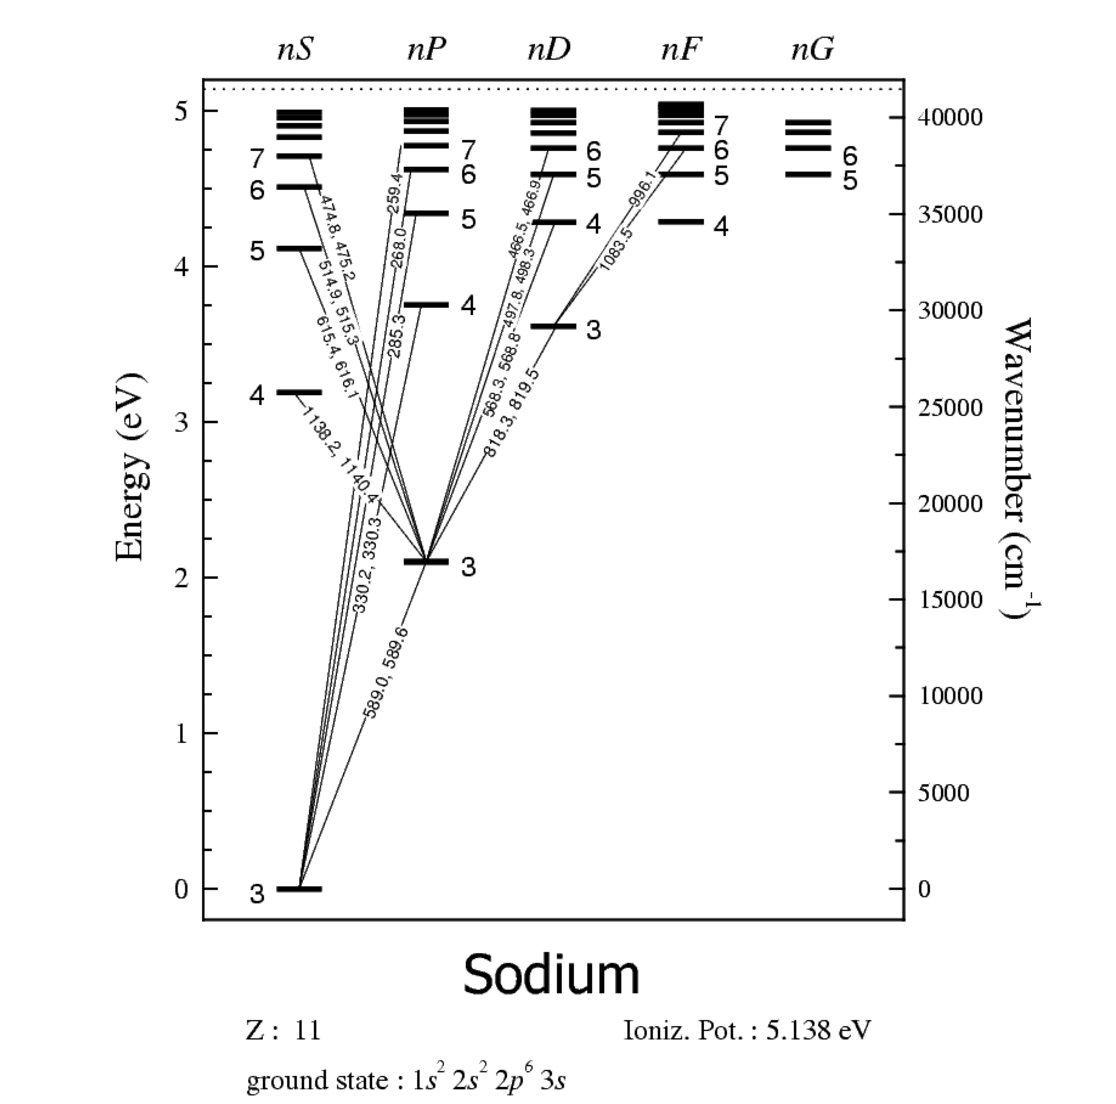
\includegraphics[scale = .50]{Images/sodiumtransition.png}
%  \caption{Figure of the energy levels of sodium, showing the possible transitions in energy the atom can make \protect\cite{sodiumlevels}.}
%  \label{fig:sodiumtransition}
%\end{figure}


These transitions are the basis for the absorption and emission of light by atoms. Photons have an associated energy
\begin{equation}
  E = h f = \frac{hc}{\lambda},
  \label{energyfrequency}
\end{equation}
%
where $f$ is the frequency of the photon, $\lambda$ is the wavelength of the photon, and $c$ is the speed of light. Thus, an atom can absorb a photon that has an energy equal to the energy difference between any of the energy levels described previously,\footnote{There are other rules governing absorption and emission besides conservation of energy which will be addressed.} and transition into a higher energy state. Furthermore, an atom can also lower its energy be emitting a photon equal to the energy difference between any two energy levels. This is the process by which sodium laser guide stars function: laser light with energy equal to the energy difference between two levels in sodium is shone upon sodium in the atmosphere where it is absorbed and then emitted in random directions, creating a ``globe'' of light (see Appendix A for more discussion on laser guide stars).



For sodium, the ground state is split into two levels, creating two distinct transitions, from $3\text{S}_{1/2}$ to $3\text{P}_{3/2}$ and $3\text{S}_{1/2}$ to $3\text{P}_{1/2}$ \cite{Kibblewhite2009}, where S and P refer to the orbital angular momentum quantum number values of $L = 0,1$, respectively, the number in front refers to the principal quantum number $n$, and the subscript refers to the total angular momentum quantum number. These transitions have respective wavelengths of $\SI{588.99}{\nano\meter}$ and $\SI{589.59}{\nano\meter}$ \cite{Kibblewhite2009}. For rubidium 87 (the atom we will be using), the transition between the $5\text{S}_{1/2}$ to $5\text{P}_{3/2}$ has a wavelength of $\SI{780.24}{\nano \meter}$ \cite{steck}. This rubidium transition, as well as the $3\text{S}_{1/2}$ to $3\text{P}_{3/2}$ transition of sodium, is known as the $\text{D}_2$ transition. 





%%%%%%%%%%%%%%%%%%%%%%%%%%%%%%%%%%%%%%%%%%%%%%%%%%
% Magnetic Resonant Pulsing
%%%%%%%%%%%%%%%%%%%%%%%%%%%%%%%%%%%%%%%%%%%%%%%%%%
\section{Magnetic Resonant Pulsing}


One technique that is often used in LGS to increase atomic fluorescence is the use of circularly polarized laser light, which is light with an electric field rotating along a circular path. Photons in circularly polarized light carry spin angular momentum (SAM), and due to conservation of angular momentum, this momentum is imparted onto the atom upon absorption. When an atom absorbs a photon with SAM of $S_z = + \hbar$, the angular momentum of the atom must increase by the same amount, so $\Delta m_F = + 1$. Then, upon emitting a photon, the atom can decay to any state satisfying $\Delta m_F = \pm 1, 0$. However, no matter which state the atom decays into, it will again be pumped back up with $\Delta m_F = +1$. Hence, atoms tend to move towards states of higher angular momenta and eventually end up in a cycling transition between the states of highest angular momenta. This process, shown in Fig. \ref{fig:opticalpumping}, is known as \textit{optical pumping} \cite{Kane2014}. By pumping all atoms into this two-level transition, we ensure that the atoms can only have one decay path with a high probability. This has been computationally simulated and shown to increase photon emission and absorption by a factor of 3 \cite{Kibblewhite2009}.

%When the D2a transition is excited by circularly polarized light at high irradiance (Wmsquared) a large fraction of atoms are pumped into the (S, F = 2, m = pm 3) substate and the atoms cycle on the transition to the (P, F = 3, m = pm3), with m the magnetic quantum number, so that sodium effectively becomes a two-level system. This process is known to create higher levels of irradiance. \cite{Holzlohner2012}

%\begin{figure}[t]
%  \centering
%  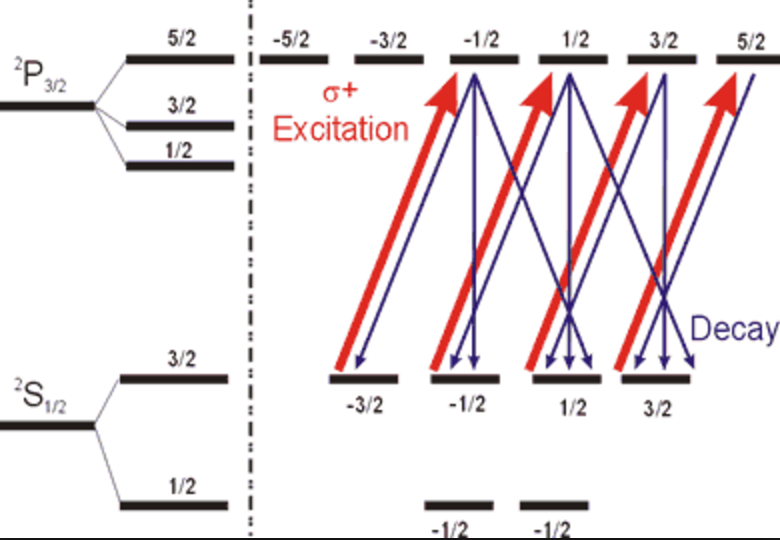
\includegraphics[scale = .75]{Images/opticalpumping.png}
%  \caption{Figure of optical pumping in which the excitation of the atom results in an angular momentum change of $\Delta m = +1$ but decay governed by $\Delta m = \pm 1, 0$ \protect\cite{opticalpumping}.}
%  \label{fig:opticalpumping}
%\end{figure}

\begin{figure}[ht]
	\centering
	\includestandalone[width = .9\textwidth]{Images/tikz/opticalpumping}
	\caption{Optical pumping in which the excitation of the atom results in an angular momentum change of $\Delta m_F = +1$ but decay governed by $\Delta m_F = \pm 1, 0$ \protect\cite{opticalpumping}.}
	\label{fig:opticalpumping}
\end{figure}



However, when exposed to an external magnetic field, the $\vec F$ vector will tend to precess about the magnetic field, in what is known as \textit{Larmor precession}. Classically, this precession can be thought of as due to the torque a magnetic field exerts on the atom

\begin{equation}
  \vec \tau = \vec \mu \times \vec B,
  \label{larmortorque}
\end{equation}
%
where $\vec \mu$ is the magnetic moment of the atom and $\vec B$ is the external magnetic field. This equation can be rewritten by noting that the magnetic moment of the atom is the product of the gyromagnetic ratio and angular momentum of the atom, i.e.

\begin{equation}
  \vec \mu = \gamma \vec F,
  \label{magneticmoment}
\end{equation}
%
where $\vec F$ is the atom's combined angular momentum and $\gamma = g\frac{e}{2m}$ is the gyromagnetic ratio with $e$ being the charge of an electron, $g$ being the g-factor, and $m$ being the mass of the atom.
%
%\begin{equation}
%  \vec \tau = \gamma \vec J \times \vec B.
%  \label{larmortorque2}
%\end{equation}
%
The angular frequency of this precession, known as the \textit{Larmor frequency}, can be found by solving $\vec \tau = \frac{d\vec F}{dt}$, leading to

\begin{equation}
  \omega_L = \gamma B.
  \label{larmorfrequency}
\end{equation}
%
From the Larmor frequency, we can compute the energy shift due to the magnetic field. This shift is
\begin{equation}
		\Delta E = \hbar \omega_L = \hbar \gamma B.
		\label{ehw}
\end{equation}
%
Larmor precession degrades the benefits obtained by optical pumping. Optical pumping relies on redistributing the angular momentum of the atom until a cycling transition is established. However, for an atom in a magnetic field not aligned with the direction of the laser beam, this cycling transition cannot be established since the angular momentum of the atom is changing in time as the magnetic field reorients $\vec F$. Typically, the magnetic field reorients the atom much faster than the benefits of optical pumping can be obtained \cite{Kane2014}. Thus, the increase in absorption and emission typically gained with optical pumping is greatly reduced for atoms exposed to a magnetic field.


%Concerned with high luminosity 

%F is the total atomic angular momentum quantum number

However, if we substitute the energy shift from the Zeeman effect, given by Eq. \ref{zeeman}, into Eq. \ref{ehw}, we can find the frequency of the atom's precession in terms of known quantities

\begin{equation}
	\omega_L = \frac{\mu_B m_F g_F}{\hbar} B.
  \label{zeemanf}
\end{equation}
%
Instead of pumping the atoms continuously with light (using a CW laser), we can optically pump the atoms with light that is pulsed at a repetition rate equal to this frequency $\omega_L$. This allows the light to only ``talk'' to the atoms at one point in the precession cycle, as if the atom were not precessing at all. The benefits of optical pumping can be reestablished with this technique, since a cycling transition can be reached without the combined angular momentum $\vec F$ changing in time. This technique is known as \textit{magnetic resonant pulsing} \cite{Kane2014}.\footnote{The idea of magnetic resonant pulsing is analogous to pushing a child on a swing. If you apply a constant force the whole time, your child will not establish a nice swinging oscillation. However, if you give a good push at one point each oscillation, your child will soon be swinging quite high.}


In this chapter, we have described the necessary theory that underpins this thesis. We have explained the quantum theory of laser guide stars and magnetic resonant pulsing. In the following chapters, we will discuss our experimental setup, methods, and results to test the effects of magnetic resonant pulsing, as well as explain theoretical ideas when necessary.
